\chapter{METODE PENELITIAN}

\section{Tahapan Penelitian}

Tahapan penelitian dalam skripsi ini melalui tahapan sebagai berikut.

\begin{enumerate}
	\item Tahap pengumpulan data, kegiatan yang dilakukan pada tahap pertama adalah peneliti mengumpulkan data. Pada tahap ini peneliti juga mencari informasi data, yaitu membaca artikel penelitian sebelumnya yang berkaitan dengan MTSP dan juga menyiapkan alat bantu atau aplikasi yang akan digunakan untuk membantu pengolahan data. Dari tahap ini data akan dikumpulkan kemudian dilanjutkan ke tahapan selanjutnya.
	\item Tahap pengolahan data, pada tahap ini penulis mulai mengolah data yang telah dikumpulkan sebelumnya untuk diolah dan dari tahap ini akan dilakukan uji coba untuk mengetahui keefektifan metode yang digunakan.
	\item Tahap analisis, setelah mendapatkan hasil uji coba peneliti mulai menganalisis hasil, menjabarkan, serta mengevaluasinya.
	\item Tahap implementasi, pada tahap terakhir ini penelitian yang telah dievaluasi dapat digunakan dan diterapkan pada tempat penelitian.
\end{enumerate}

\section{Prosedur Penelitian}


\subsection{Data Penelitian}
    
Berdasarkan studi kasus dalam skripsi ini, data yang akan digunakan dalam penelitian ini adalah data koordinat dari seluruh SMA di Kabupaten Probolinggo. Data nama-nama sekolah dikumpulkan dari \url{https://referensi.data.kemdikbud.go.id/} \cite{kemendikbud}, dan data koordinat dikumpulkan melalui aplikasi Google Earth \cite{googleearth} yang dapat diunduh langsung ke dalam bentuk \textit{spreadsheet}, dapat dilihat pada Lampiran \ref{lampiran1}. Waktu yang diperlukan peneliti untuk mengumpulkan data dari web tersebut kurang lebih sekitar satu bulan.

\subsection{Instrumen Pendukung}
\begin{enumerate}
    \item Python
    
    Dalam penelitian ini akan digunakan bahasa pemrograman python untuk mempermudah pengerjaan. Bahasa python adalah bahasa pemrograman baru di masa sekarang, karena dalam bahasa ini lebih simpel dan singkat dalam membuat program \cite{syahrudin2018input}. Bahasa pemrograman ini merupakan bahasa pemrograman yang paling mudah dipelajari dari pada bahasa pemrograman yang lain. Serta dalam bahasa pemrograman ini dapat menjalankan beberapa rumus matematika di dalamnya. Selain itu bahasa Python telah digunakan secara luas, dan masuk dalam 3 besar bahasa pemrograman yang digunakan dalam beberapa tahun belakangan.
    
    \item Jupyter Notebook
    
    Jupyter Notebook adalah aplikasi web gratis yang digunakan untuk membuat dan membagikan dokumen komputasi, hasil hitungan, visualisasi, dan teks \cite{Kluyver2016jupyter}. Notebook ini juga mendukung 3 bahasa pemrograman salah satunya adalah bahasa pemrograman python. Banyak kelebihan yang disajikan dari aplikasi ini salah satunya adalah mendokumentasikan kode, dan menjalankan kode dalam setiap sel, dan visualisasi data seperti pada Gambar \ref{fig:visjupyter}.

\begin{figure}[H]
  \centering
  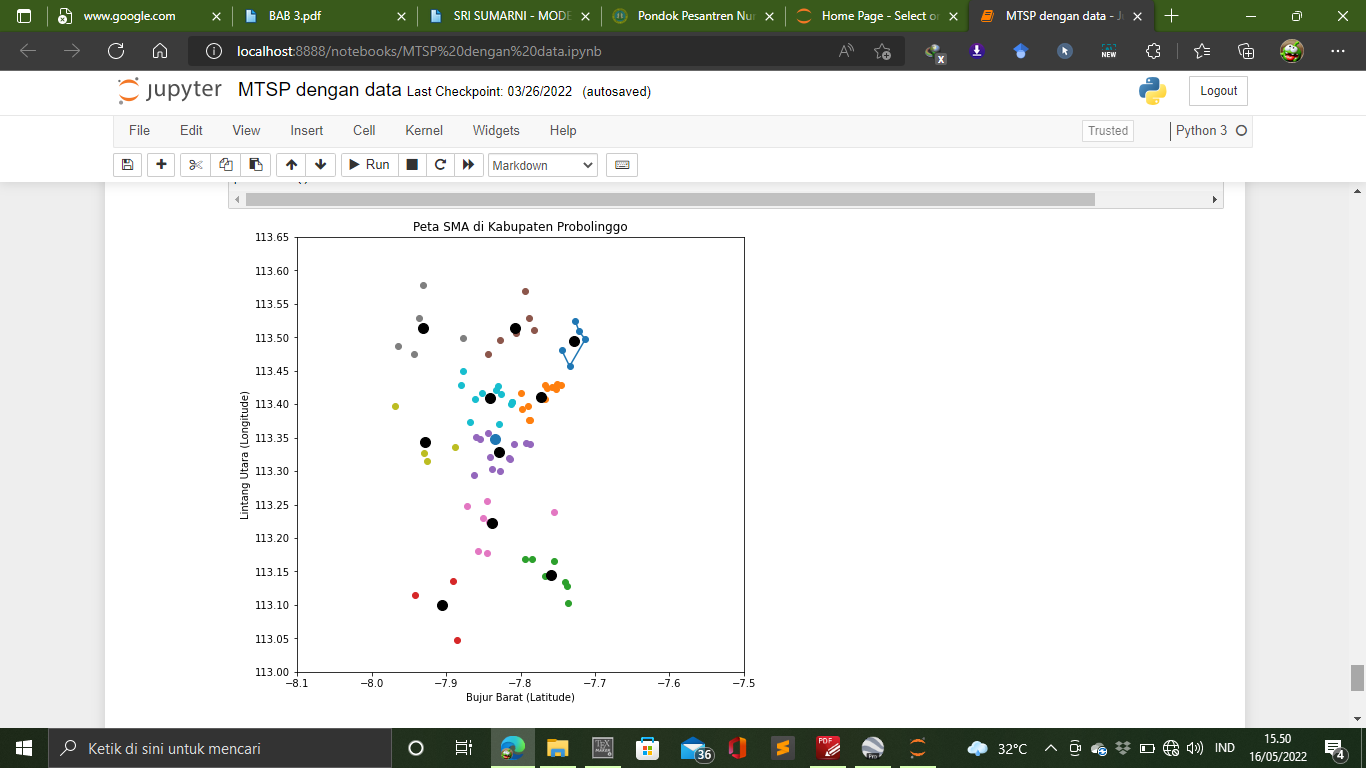
\includegraphics[width=0.8\textwidth]{Gambar/visualisasi jupyter.png}
  \caption{Visualisasi data jupyter notebook}
  \label{fig:visjupyter}
\end{figure}

	\item Google Earth
	
	Google Earth digunakan dalam penelitian ini untuk mengumpulkan koordinat lokasi seluruh SMA di Kabupaten Probolinggo. Aplikasi ini dapat menandai beberapa lokasi secara langsung seperti pada Gambar \ref{fig:markloc} dan mengekspor ke dalam bentuk spreadsheet seperti pada Gambar \ref{fig:eksspread}. Data-data lokasi yang telah diunduh ke dalam bentuk spreadsheet akan diproses menggunakan jupyter notebook.

\begin{figure}[H]
  \centering
  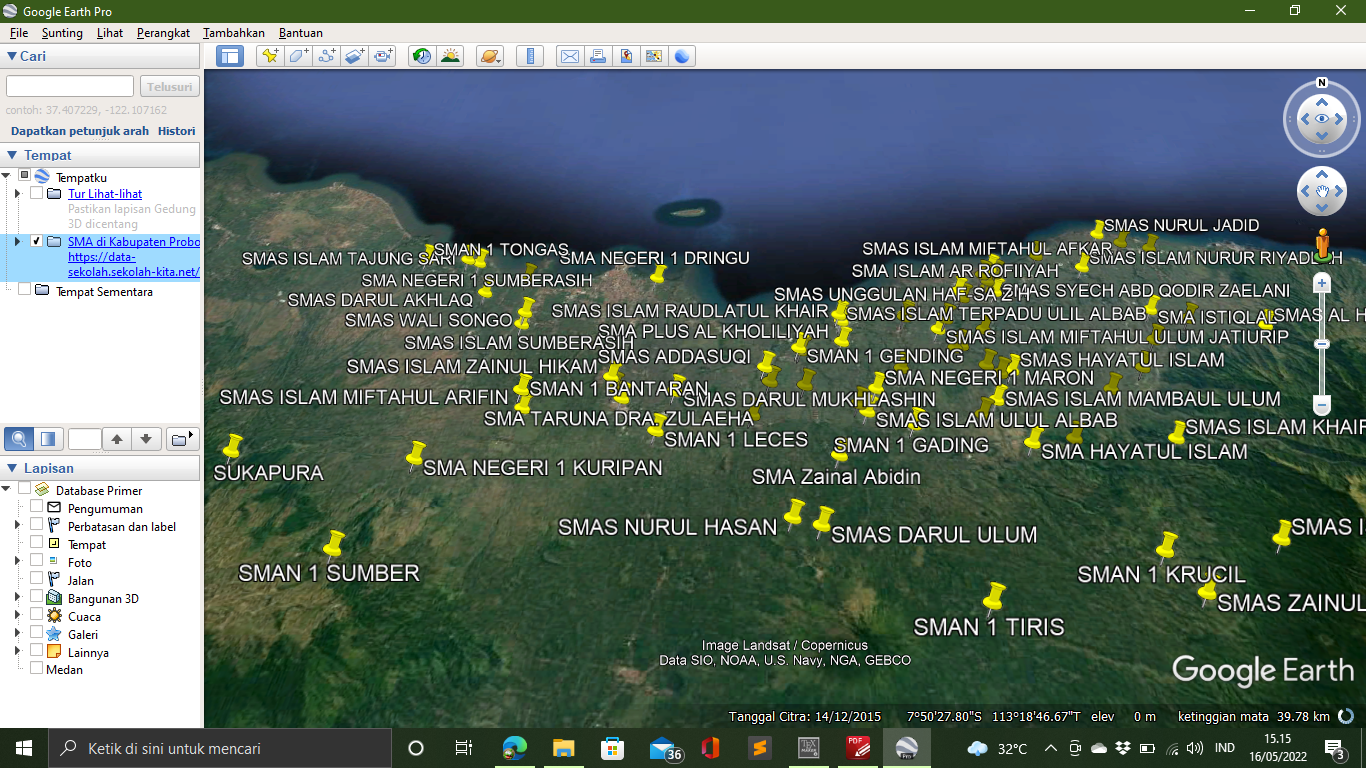
\includegraphics[width=0.8\textwidth]{Gambar/google earth.png}
  \caption{Menandai lokasi pada Google Earth}
  \label{fig:markloc}
\end{figure}

\begin{figure}[H]
  \centering
  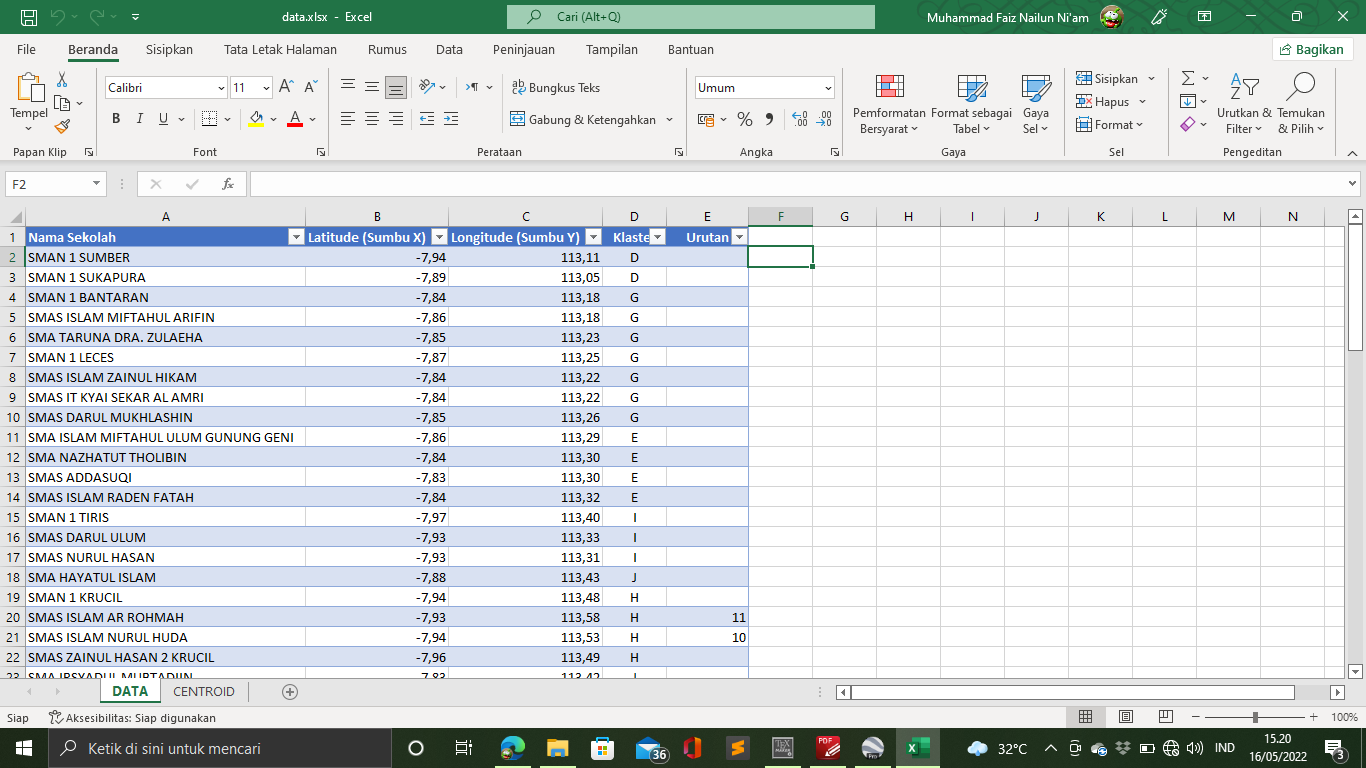
\includegraphics[width=0.8\textwidth]{Gambar/ekspor spreadsheet.png}
  \caption{Mengekspor data ke bentuk spreadsheet}
  \label{fig:eksspread}
\end{figure}

\end{enumerate}

\subsection{Langkah-langkah Dalam Tahap Pengolahan Data}
\begin{enumerate}
    \item Peneliti menyiapkan data yang telah dikumpulkan sebelumnya.
    \item Selanjutnya peneliti melakukan pengelompokkan data sebanyak 1 sampai dengan 10 klaster, untuk menemukan pembagian klaster sekaligus rute yang paling optimal. Metode yang digunakan adalah algoritma \textit{k}-means, dengan langkah-langkah sebagai berikut.
    \begin{enumerate}
        \item Pilih titik-titik \textit{centroid} sesuai banyak klaster
        \item \label{ulang1} Hitung jarak tiap titik tujuan dengan masing-masing \textit{centroid} dengan rumus \textit{Euclidean distance} seperti pada Persamaan (\ref{eq:euclidean}).
        \item Setelah seluruh titik dimasukan ke dalam klaster, hitung \textit{centroid} baru dengan cara menghitung rata-rata titik pada klaster tersebut. Lakukan hal yang sama pada klaster yang lain.
        \item Ulangi langkah \ref{ulang1} sampai tidak ada perubahan pada anggota klaster.
    \end{enumerate}
	
	\item Selanjutnya melakukan proses pencarian rute terpendeknya atau TSP pada setiap klaster yang telah dibagi, langkah-langkahnya adalah sebagai berikut.
	\begin{enumerate}
		\item Bangkitkan populasi awal yang berisi sejumlah kromosom
	    \item \label{ulang2} Hitung nilai \textit{fitness} (jarak) tiap kromosom
	    \item Tetapkan probabilitas \textit{crossover} ($p_c$) dan bangkitkan bilangan acak (0,0000 sampai 1,0000) pada tiap kromosom, jika bilangan acak kurang dari $p_c$ maka dilakukan \textit{crossover}. Jika \textit{fitness} kromosom hasil \textit{crossover} lebih baik dari kromosom awal, maka kromosom awal digantikan dengan kromosom hasil \textit{crossover}.
	    \item Tetapkan probabilitas mutasi ($p_m$) dan bangkitkan bilangan acak (0,0000 sampai 1,0000) pada setiap kromosom. Jika bilangan acak kurang dari $p_m$ maka akan dilakukan mutasi. Kromosom awal digantikan dengan kromosom hasil mutasi jika kromosom hasil mutasi memiliki fitness yang lebih baik dari kromosom awal.
	    \item Jika hasil kurang optimal, iterasi dilakukan dengan cara kembali ke tahapan \ref{ulang2} untuk generasi berikutnya sampai hasil yang dilakukan optimal atau mendekati optimal.
    \end{enumerate}
	\item Ketika proses diatas selesai dilakukan maka dihasilkan pembagian klaster dan rute terdekat tiap klaster menuju seluruh SMA di Kabupaten Probolinggo
	\item Mengevaluasi data yang dihasilkan
\end{enumerate}